\section{Introduction}
    Inverse photoemission spectroscopy (IPES) is an experimental technique used in condensed matter physics to map the unoccupied electronic structure
    of a material. In an ultra-high vacuum environment, a beam of electrons of known energy is impinged on a sample. If the energy of the incoming
    electrons align with a state which lies above the fermi energy, then they will couple to that state. Detections come from photons released through
    radiative relaxation of these excited states, which are in the UV range for typical electron energies of 10-100eV. We are able to map the unoccupied states
    by recording the number of photon detections we obtain at a given incident electron energy. In order to obtain significant IPES results a spectrometer must meet strict requirements of both its photodectors and its electron source. Our previous efforts in 
    spectrometer characterization focused on its photodetection capabilities. In this report we detail our work to characterize the performance 
    of our electron source.

    The electron source, also referred to as an electron gun, must be capable of operating within at low electron energies while still producing a beam with a minimal spot size and 
    momentum spread. The current of electrons reaching the sample should also be as large as possible, equivalent to the gun having a high brightness. Achieving this is a highly 
    non-trivial due to the contradictory requests of being low energy but also high brightness\cite{stoffel1985low}. Emission current limitations in these type of guns are caused by the space charge effect, 
    where the cloud of low energy electrons that make up the beam repel incoming electrons back towards the source\cite{staib}. Commercially available 
    electron guns are capable of meeting these requirements and thus solve the problem of needing to carefully balance these two main considerations; however they introduce a 
    new problem in that one is now tasked with finding the operating conditions of the gun which allows it to do so. The electron gun in our spectrometer has 10 unique parameters
    which can each be varied by applying a voltage bias. So to obtain a high brightness beam which operates at low energies we need to determine a combination of these 10 
    voltages, an optimization problem that is made exceedingly difficult by this large parameter space. 

    Starting with the configuration recommended by our electron gun's manufacturer we measured the beam width and maximum current. The beam was found 
    to be insufficient for use in IPES, which was attributed to space charge limiting. Reducing the temperature of the gun's cathode allowed us 
    to remove a parameter from the optimization problem, and yielded much better results in subsequent tests. Further constraints were placed on the 
    possible configurations which could use for the gun, which again reduced the difficulty of the optimization problem. Eventually a set of parameters 
    was found, which produced a beam of gaussian profile with a small spot size and divergence angle, on par with what has been reported by other groups\cite{ipes,raj2004optimization,stoffel1985low,budke}.
    Subsequent calculations showed that this beam is able to resolve the first brillouin zone of copper. Our spectrometer is now in a condition where 
    only minor work needs to be carried out before we are able to produce meaningful IPES results.


\section{Inverse Photoemission Spectroscopy}

\subsection{The Inverse Photoemission Process}

A useful way to understand inverse photoemission is to think of it in the context the photoelectric effect. Photons incident on the surface of a sample with a sufficiently
large energy will lead to the liberation of electrons. The determining factor in this process is if the photon has an energy greater than or equal to the sample's work function, which 
is defined as the energy difference between the sample's fermi level and vacuum level. The fermi level is the highest energy occupied electronic state, and the 
vacuum level is the energy of a free electron above the sample's surface. Inverse photoemission is the dual of this process, where instead a beam of electrons incident on a sample 
leads to the emission of photons through radiative decay. 

The mechanism through which this occurs starts with the electron coupling to an unoccupied electronic state with an energy that matches its initial energy, the state must be unoccupied in 
order to satisfy the Pauli principle. This unoccupied state is of a relatively high energy compared to the fermi energy, meaning that the sample remaining in this configuration 
is energetically unfavourable. As a result the electron decays to a lower energy unoccupied state, and the energy difference between the two states is what determines the energy of 
the emitted photon. It should be noted that at this electron energy range the penetration depth of electrons into a sample is at its minimum\cite{penn1987electron},
making IPES a very surface sensitive technique.

There are two ways to use this process for spectroscopy. In the first, the electron energy is varied and only photons of a single frequency are detected. 
In the second, the electron energy is fixed and the full range of emitted photons is collected. These modes are known as isochromat and spectrograph respectively; our system operates in the isochromat 
mode so we will limit the scope of further discussion to reflect this. 

\subsection{Energy Conservation in Inverse Photoemission}

In isochromat mode we vary the energy of electrons and record the intensity of photons with a set frequency $\omega_0$, thus the electron can only decay to states which meet the requirement that:

\begin{equation}
    E_i = \hbar\omega_0 + E_f
\end{equation}

Which means that if we know $E_i$ and $\omega_0$ then we can determine the energy of the unoccupied state $E_f$. So IPES allows us to map all of the $E_f$ states by varying $E_i$ and 
recording photon intensity. In general determining $E_i$ is a difficult task, since it is defined as:

\begin{equation}\label{vg}
    E_i = eV_g + \Phi_g
\end{equation}

where $V_g$ is the voltage applied to the electron gun's cathode, and $\Phi_g$ is the work function of the cathode. The difficulty comes from the fact that we don't know $V_g$ to great 
precision, and don't have a value for $\Phi_g$ at all. We can overcome this by measuring $E_f$ relative to the fermi energy, so for example if we get a peak in our spectrum at 
$E_f = 5\textrm{eV}$, then we know that there is an unoccupied state at an energy of 5eV above the fermi level. As we will later see however, 
this approach is insufficient if we want to perform what is called an angle resolved measurement on the sample. In this case we need to know the 
momentum of the electrons reaching the sample, and doing so requires a knowledge of the kinetic energy of the electrons which depends on $E_i$. 

\subsection{Momentum Conservation}

At the scale of an electron incident on a macroscopic sample, there is essentially infinite translational symmetry in the directions parallel to the sample's surface.
This symmetry means the electron's momentum in those parallel directions must be conserved as it changes from being a free electron to being bound 
in one of the sample's energy levels. This adds a further requirement that the momentum of the states to which the electron couples and decays into must match its initial parallel momentum. 
If we consider the kinetic energy of a free electron\cite{ipes}, just before it is bound to the sample we have:

\begin{equation}
    E_k = \frac{\hbar^2 k^2}{2m_e}
\end{equation}

Solving for the magnitude of the electron's momentum and we get:

\begin{equation}
    k = \frac{\sqrt{2m_e E}}{\hbar}
\end{equation}

If we define $\theta$ as the angle between the beam's axis and the samples surface, then the parallel component of the momentum is given by:

\begin{equation}\label{kpar}
    k_\parallel = k\sin{\theta}
\end{equation}

So by changing the incidence angle of the electron beam we are able to select states with the same $E_i$ value but with a different $k_\parallel$, letting us probe much more of 
the band dispersion. This technique is known as angle- or k-resolved inverse photoemission spectroscopy (KRIPES) and is one of the biggest selling points of the IPES method. 

\subsection{The Contact Potential}

Similarly to $E_i$, determining a value for $E_k$ is equally difficult since it is defined as:

\begin{equation}
  E_k = E_i - \Phi_s
\end{equation}

Where $\Phi_s$ is the work function of the sample undergoing inverse photoemission. If we insert equation \eqref{vg} we find that:

\begin{equation}
  E_k = eV_g + \Phi_g - \Phi_s
\end{equation}

We define the contact potential, $\Delta$, to be:

\begin{equation}\label{delta}
  \Delta = \Phi_s - \Phi_g
\end{equation}

Which tells us that the kinetic energy of the incident electrons is given by:

\begin{equation}\label{Ek}
  E_k = eV_g - \Delta
\end{equation}

Since $\Delta$ is dependent on the work function of the sample, its exact value will change for every sample we study with IPES. Determining a value for $\Delta$ can thankfully be
done by following a simple procedure\cite{mcmahon_2012}. With the electron beam incident on a sample with a known energy, we apply a bias voltage to the sample and record the 
resulting sample current. With an increasing sample bias, the current should remain mostly constant until reaching a threshold value where the current rapidly drops to zero. Keeping 
the sample bias voltage and gun cathode voltage in mind we consider the required $V_g$ to overcome the potential barrier created by having $\Phi_s > \Phi_g$:

\begin{equation}
  V_g = \frac{\Phi_s - \Phi_g}{e}
\end{equation}

If we now apply an arbitrary bias voltage to the sample the cathode voltage needs to increase to:

\begin{equation}
  V_g = V_s + \frac{\Phi_s - \Phi_g}{e}
\end{equation}

Inserting equation \eqref{delta} and solving yields:

\begin{equation}\label{vgvs}
  \Delta = e(V_g - V_s)
\end{equation}

Thus using the cathode voltage and the threshold bias voltage we recorded, we can determine the contact potential and from that determine the kinetic energy of the electrons in beam.

\section{The Electron Gun}

\subsection{Thermionic Emission}

The electron gun used in our spectrometer is a thermionic emission type. In this design, a heated cathode is used as the source of electrons. The 
high temperature of the filament allows for electrons in the cathode to be thermally excited to its vacuum level. Low work function cathodes 
are chosen to reduce the operating temperature needed to excite the same amount of electrons. In the case of our electron gun, this is achieved by 
using a BaO coated filament which has a lower work function than the same filament without a coating\cite{kimballphysics}. The current density 
emitted from the cathode at a temperate $T$ and work function $\Phi$ is given by Richardson's Law:

\begin{equation}\label{richardson}
  J = A_G T^2 \mathrm{e}^{-\frac{\Phi}{kT}}
\end{equation}

Where $A_G$ is the cathode material's Richardson constant. From this we see that emission current is inversely proportional to work function, and 
proportional to cathode temperature. Thus we can obtain a comparable current to a hot, high work function cathode using a colder and lower work function 
cathode. A gun operating at these reduced temperatures will have a longer cathode lifetime, and is generally referred to as being in the temperature limited 
mode.

\subsection{Space Charge Effect}

When working with low energy electron beams, the space charge effect has a much greater impact on maximum achievable beam currents than 
high energy counterparts\cite{staib,stoffel1985low,raj2004optimization}.
As electrons are emitted from the filament, they form a space charge which will eventually form the beam. As the charge of this distribution increases, 
its repulsive force can send electrons back to the filament. It can further prevent electrons from leaving the filament in the first place. The current 
density of a space charge limited cathode is given by Child's Law:

\begin{equation}
  J = K \frac{V_d^{3/2}}{d^2}
\end{equation}

Where K is a constant, $V_d$ is the potential difference between the cathode and anode, and $d$ is the cathode to anode distance.
We notice that unlike Richardson's law, there is no longer a temperature dependence for our current density, meaning that a space charge limited
beam is resistant to temperature fluctuations. However, space charge limiting only becomes a significant factor at high cathode temperatures, 
after the gun moves out of the temperature limited mode.

\clearpage
\subsection{Electron Gun Construction}

\begin{figure}[h!]
  \centering
  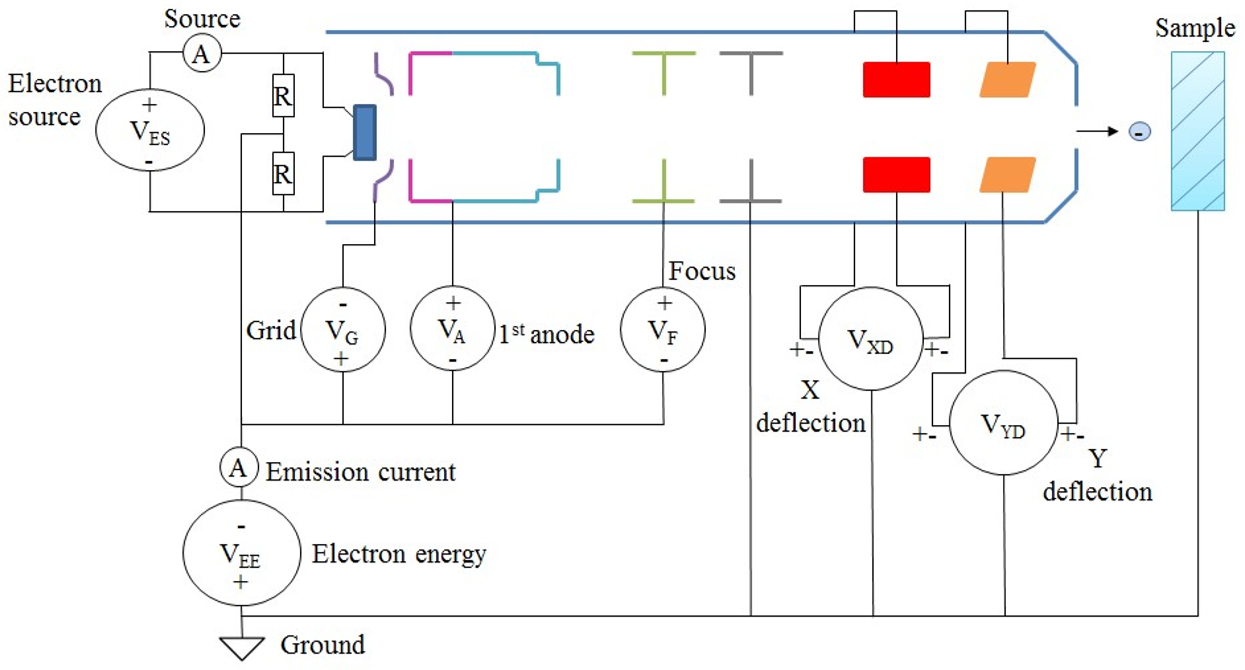
\includegraphics[width=0.85\linewidth]{../Assets/Gun diagram.png}
  \caption{Block Diagram of thermionic emission type electron gun for use in low energy applications\cite{gina_2012}}
  \label{fig:egun}
\end{figure}

Figure \ref{fig:egun} shows a typical design for low energy electron guns which use a heated cathode. The ground of the electron gun is connected 
to the supply which controls electron energy, meaning that all potentials are going to be floated by whatever potential is selected for electron energy. 
The sample and gun assembly share the same ground, meaning that the gun's potentials are also floating with respect to the sample. 

The filament supply voltage controls the temperature of the cathode, and is limited to a range of 0V to 5V. The temperature is increased through ohmic heating and an emission 
current is generated through thermionic emission. The electrons are accelerated through the gun by the extraction potential (labeled first anode in figure \ref{fig:egun}),
which is limited to a range of 0V to 100V. After being pulled from the cathode the electrons pass through the grid, which controls the brightness of the beam. 
It can be biased with a potential between -15V and 15V, a sufficiently negative grid voltage can suppress the emission of electrons entirely. The shaping
of the beam is done by the focusing electrodes. Our gun has two separate electrodes which can be independently biased in a range determined by the electron 
energy and extraction potential. Finally, the beam can be steered in the two directions perpendicular to its axis by using two parallel plate deflectors. 
This can be used to realign the beam towards the sample if it is found to be deflecting off target. 

The goal in characterizing an electron gun is to find a combination of all of these parameters which meet the strict requirements of inverse 
photoemission. A notable thing to balance is the cathode temperature and extraction voltage, as it controls if the gun is operating in the temperature limited 
or space charge limited regime. In the temperature limited regime we have longer filament lifetimes and a potential for larger sample currents, but 
the emission current is highly dependent on cathode temperature. Space charge limiting provides us stability in emission current but at the cost of 
a hot filament with a much lower lifetime and maximum emission. Best results are obtained when there is some balance between the two, yielding a stable and sufficiently high 
emission current, while also prolonging cathode lifetime\cite{stoffel1985low,staib}. Other considerations include keeping the focus potential to roughly the same order as the extraction 
potential, which minimizes the amount of accelerating and decelerating an electron in the beam undergoes, which is more likely to provide a well 
behaved beam\cite{stoffel1985low,raj2004optimization}.